\documentclass[tikz,border=3pt]{standalone}
\usepackage{amsmath,lmodern}
\usetikzlibrary{arrows.meta,positioning,calc}
\definecolor{Ink}{HTML}{163047}
\definecolor{Teal}{HTML}{087F8C}
\definecolor{Clay}{HTML}{AD4C2B}
\begin{document}
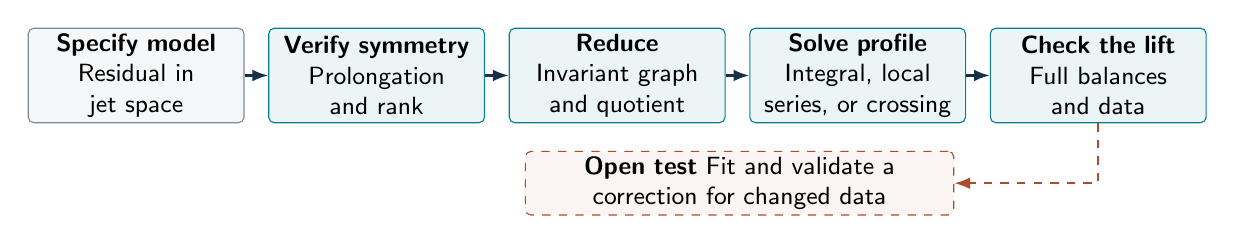
\begin{tikzpicture}[font=\sffamily\small,box/.style={draw=Ink!56,fill=Ink!4,rounded corners=2pt,align=center,text width=26mm,minimum height=12mm,inner sep=2pt},
gate/.style={box,draw=Teal,fill=Teal!8},open/.style={box,draw=Clay,dashed,fill=Clay!6},flow/.style={-{Latex[length=2mm]},draw=Ink,thick}]
\node[box] (eq) {\textbf{Specify model}\\Residual in jet space};
\node[gate,right=3mm of eq] (sym) {\textbf{Verify symmetry}\\Prolongation and rank};
\node[gate,right=3mm of sym] (q) {\textbf{Reduce}\\Invariant graph and quotient};
\node[gate,right=3mm of q] (profile) {\textbf{Solve profile}\\Integral, local series, or crossing};
\node[gate,right=3mm of profile] (lift) {\textbf{Check the lift}\\Full balances and data};
\draw[flow] (eq)--(sym);
\draw[flow] (sym)--(q);
\draw[flow] (q)--(profile);
\draw[flow] (profile)--(lift);
\node[open,below=3.5mm of profile,xshift=-15mm,text width=53mm,minimum height=8mm] (cor) {\textbf{Open test} Fit and validate a correction for changed data};
\draw[flow,draw=Clay,dashed] (lift.south) |- (cor.east);
\end{tikzpicture}
\end{document}
